\section{Auswertung}
\label{sec:Auswertung}

Die Messwerte werden nach der chronologischen Reihenfolge der Durchführung ausgewertet. Dabei wird die Auswertung aufgeteilt
in die Bestimmung der Kraftflussdichte und die Bestimmung der effektiven Masse.

\subsection{Bestimmung der Kraftflussdichte}
\label{sub:Kraftflussdichte}

Als erstes werden die aufgenommenen Daten der Magnetfeldstärke gegen den Ort aufgetragen.
Dies ist in \autoref{fig:plot1} dargestellt.
\begin{figure}[H]
  \centering
  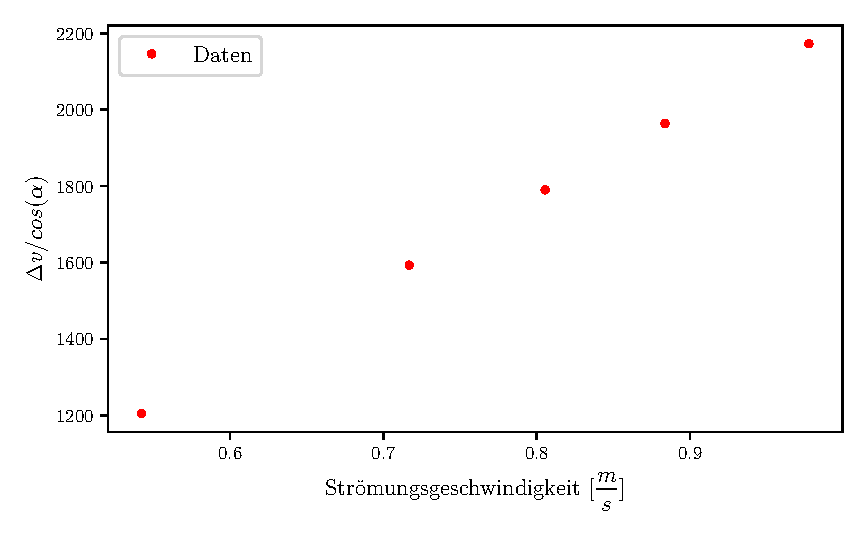
\includegraphics[width=\textwidth]{build/plot1.pdf}
  \caption {Magnetfeldstärke in Abhängigkeit der Position der Hall-Sonde.}
  \label{fig:plot1}
\end{figure}


Die maximale Kraftflussdichte entspricht der Feldstärke am Ort der Probe.
Somit liegt die Feldstärke im Bereich der Probe bei 
\begin{align*}
  B &= \qty{435}{\tesla}
\end{align*}

\subsection{Bestimmung der effektiven Masse}
\label{sub:effektiveMasse}

Zur Bestimmung der effektiven Masse werden die durch die Messung bestimmten Winkel unter denen ein Minimum der Signalamplitude gefunden wurde
normiert, also durch die Länge $L$ der Probe geteilt.
Dadurch, dass das Feld bei der Umpolung um insgesamt $\num{2}B$ geändert wird, ergibt sich der Winkel $\theta$ um den die Polarisationsebene
gedreht wurde zu
\begin{align}
  \theta &= \frac{1}{2L}(\lvert \theta_1-\theta_2 \rvert).
\end{align}
Die Dicken der Proben entsprechen der Durchlauflänge $L$ und betragen für die verwendeten Proben
\begin{align*}
  L_{\text{undotiert}}&= \qty{5.11}{\milli\meter}\\
  L_{1,2}&= \qty{1.36}{\milli\meter}\\
  L_{2,8}&= \qty{1.296}{\milli\meter}.
\end{align*}
Die Dotierungen der Proben betragen
\begin{align*}
  N_{1,2}&= \qty{1.2 e24}{\per\cubic\meter}\\
  \shortintertext{und}\\
  N_{2,8}&= \qty{2.8 e24}{\per\cubic\meter}.
\end{align*}

In \autoref{fig:plot2} sind die normierten Winkel der hochreinen Probe gegen das Quadrat der Wellenlängen der verwendeten Interferenzfilter aufgetragen.
\begin{figure}[H]
  \centering
  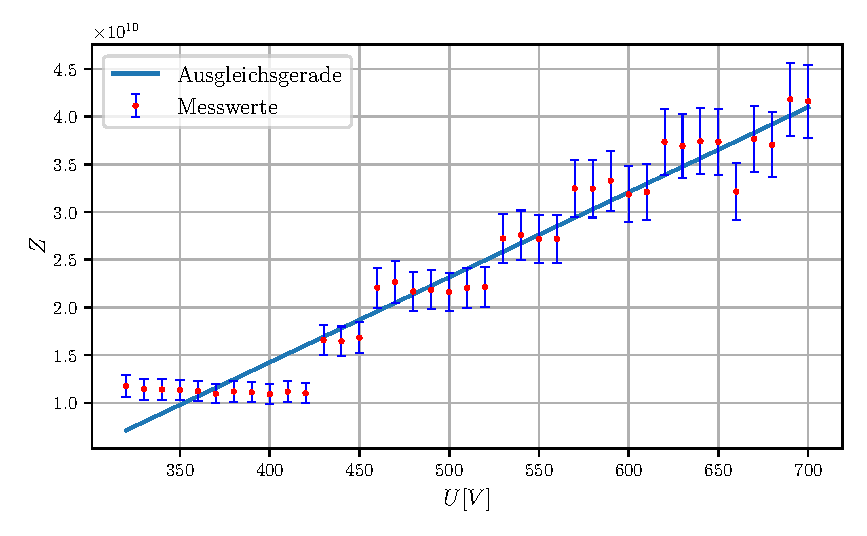
\includegraphics[width=\textwidth]{build/plot2.pdf}
  \caption {Die normierten Drehwinkel der Faraday-Rotation in Abhängigkeit von der quadrierten Wellenlänge der Interferenzfilter bei der Messung der undotierten Probe.}
  \label{fig:plot2}
\end{figure}

Um die durch die Leitungselektronen bedingte Faraday-Rotation $\theta_{\text{frei}}$ zu bestimmen, wird von den normierten Winkeln der dotierten Proben jeweils
die Faraday-Rotation der undotierten Probe abgezogen.
Die so berechneten Werte sind in \autoref{fig:plot3}
wiederum gegen die quadrierten Wellenlängen der Interferenzfilter aufgetragen.
\begin{figure}[H]
  \centering
  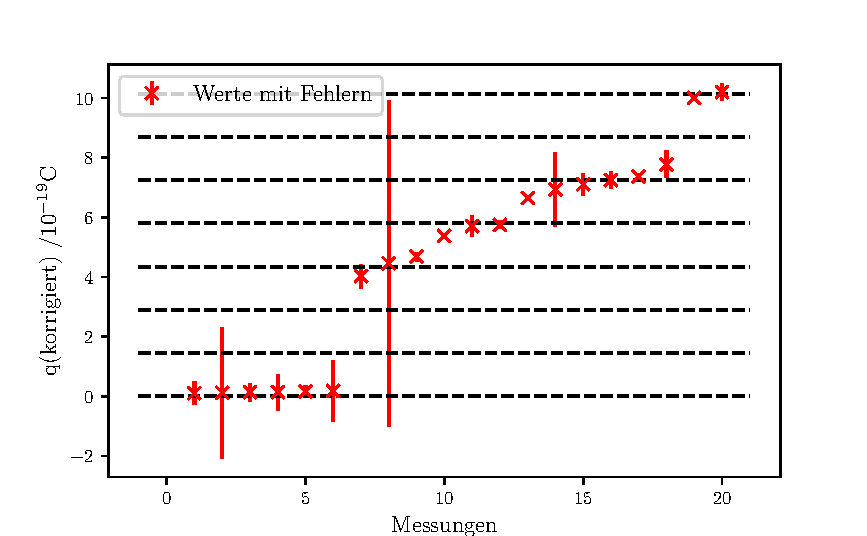
\includegraphics[width=\textwidth]{build/plot3.pdf}
  \caption {Der durch die Leitungselektronen hervorgerufene normierte Drehwinkel der Faraday-Rotation in Abhängigkeit von der quadrierten Wellenlänge der Interferenzfilter bei der Messung der dotierten Proben.}
  \label{fig:plot3}
\end{figure}
Die in orange und hellblau markierten Messwerte weichen vom Verlauf stark ab und werden daher für die Rechnung vernachlässigt.
Außerdem wird für beide Dotierungen ein Fit der Form
\begin{align*}
  \theta_{\text{frei}} &= A \cdot \lambda^2+b
\end{align*}
hinzugefügt, wobei $A$ zu
\begin{align*}
  A_{1,2}&= \num{15.6667 \pm 6.1233 e12}\si{\per\cubic\metre}\\
  \shortintertext{und}\\
  A_{2,8}&= \num{18.5253 \pm 3.9307 e12}\si{\per\cubic\metre}
\end{align*}
ermittelt wird.
Aus der Steigung $A$ kann nun durch Umstellen von \autoref{eqn:drehwinkel} die effektive Masse nach
\begin{align*}
  m^* &= \sqrt{\frac{e_0^3\cdot N \cdot B}{A\cdot 8\pi^2\varepsilon_0 c^3 \cdot n }} 
\end{align*}
berechnet werden.
Der Brechungsindex $n$ beträgt hierbei $n_{\text{GaAs}}=\num{3.3}$ \cite{BrechungsindexGaAs}.
Somit berechnet sich die effektive Masse zu
\begin{align*}
  m^*_{1,2}&=(\num{0.052 \pm 0.010}) \cdot m_e \\
  \shortintertext{und}\\
  m^*_{2,8}&=(\num{0.072 \pm 0.008})\cdot m_e.
\end{align*}